\documentclass{llncs}

\usepackage{cite}
\usepackage{graphicx}
\usepackage{amsmath,amssymb}
\usepackage{algorithm}
\usepackage{algorithmic}
\usepackage{psfrag}


% AML bibliography references
\newcommand{\bib}[1]{/aml/home/mjg82/bib/#1}

% Better references, I think
\renewcommand{\sec}[1]{Section~\ref{sec:#1}}
\newcommand{\fig}[1]{Figure~\ref{fig:#1}}
\newcommand{\alg}[1]{Algorithm~\ref{alg:#1}}

% Mathy help
\newcommand{\parens}[1]{\!\left(#1\right)}

% Algorithmic changes
\renewcommand{\algorithmicforall}{\textbf{for each}}

%% PSO Stuff
\DeclareMathOperator{\URand}{U}
\DeclareMathOperator*{\argmin}{arg\;min}
\DeclareMathOperator*{\argmax}{arg\;max}
\DeclareMathOperator*{\arginf}{arg\;inf}
\DeclareMathOperator*{\argsup}{arg\;sup}
\providecommand{\pers}{\ensuremath{P}}
\providecommand{\neigh}{\ensuremath{N}}
\providecommand{\leftind}{\ensuremath{L}}
\providecommand{\rightind}{\ensuremath{R}}
\providecommand{\nURand}{\ensuremath{U^\neigh}}
\providecommand{\pURand}{\ensuremath{U^\pers}}
\providecommand{\ppos}{\ensuremath{\Vec{x}}}
\providecommand{\fppos}{\ensuremath{\Vec{fx}}}
\providecommand{\pvel}{\ensuremath{\Vec{v}}}
\providecommand{\nbest}{\ensuremath{\Vec{x}^\neigh}}
\providecommand{\fnbest}{\ensuremath{\Vec{fx}^\neigh}}
\providecommand{\pbest}{\ensuremath{\Vec{x}^\pers}}
\providecommand{\fpbest}{\ensuremath{\Vec{fx}^\pers}}
\providecommand{\constriction}{\ensuremath{\chi}}
\providecommand{\ncoeff}{\ensuremath{\phi^\neigh}}
\providecommand{\pcoeff}{\ensuremath{\phi^\pers}}
\providecommand{\obs}{\ensuremath{\Vec{\xi}}}
\providecommand{\ofunc}{\ensuremath{f}}
\providecommand{\swarm}{\ensuremath{swarm}}

%SpecExPSO Stuff
\providecommand{\indic}{\ensuremath{I}}
\providecommand{\specvel}{\ensuremath{\vec{V}}}
\providecommand{\specpos}{\ensuremath{\vec{X}}}
\providecommand{\leftn}{\ensuremath{\Vec{x}^\leftind}}
\providecommand{\rightn}{\ensuremath{\Vec{x}^\rightind}}
\providecommand{\caseset}{\ensuremath{\mathcal{C}}}
\providecommand{\casegen}{\ensuremath{c}}
\providecommand{\casedef}{\ensuremath{(\pbest,\nbest)}}
\providecommand{\casexn}{\ensuremath{(S,-)}}
\providecommand{\casexx}{\ensuremath{(S,S)}}
\providecommand{\casexl}{\ensuremath{(S,\leftind)}}
\providecommand{\casexr}{\ensuremath{(S,\rightind)}}
\providecommand{\casepn}{\ensuremath{(-,-)}}
\providecommand{\casepl}{\ensuremath{(-,\leftind)}}
\providecommand{\casepr}{\ensuremath{(-,\rightind)}}
\providecommand{\casepN}{\ensuremath{(-,N)}}
\providecommand{\casexN}{\ensuremath{(S,N)}}
\providecommand{\noeval}[1]{\ensuremath{#1^{-e}}}
\providecommand{\nonbest}[1]{\ensuremath{#1^{-n}}}
\providecommand{\p}{\ensuremath{p}}
\providecommand{\pset}{\ensuremath{\mathbf{p}}}
\providecommand{\s}{\ensuremath{s}}
\providecommand{\sset}{\ensuremath{\mathbf{s}}}
\providecommand{\nsset}{\ensuremath{\mathbf{ns}}}
\providecommand{\n}{\ensuremath{n}}
\providecommand{\nset}{\ensuremath{\mathbf{n}}}
\providecommand{\nnset}{\ensuremath{\mathbf{nn}}}

\title{\ \\ \LARGE\bf Speculative Evaluation in Particle Swarm Optimization%
%\thanks{Matthew Gardner, Andrew McNabb, and Kevin Seppi are with the Department
%of Computer Science, Brigham Young University, 3361 TMCB, Provo, UT 84602
%(phone: 801-422-8717; email: \{mjg82,a,k\}@cs.byu.edu).}%
}

\date{}

%\author{Matthew Gardner, Andrew McNabb, and Kevin Seppi}
\author{Author names omitted for review}

\begin{document}
\maketitle

\begin{abstract}

Particle swarm optimization (PSO) has previously been parallelized only by 
adding more particles to the swarm or by parallelizing the evaluation of the
objective function.  However, some functions are more efficiently optimized with more
iterations and fewer particles.  Accordingly, we take inspiration from 
speculative execution commonly performed in modern processors and propose what
we call speculative evaluation in PSO (SEPSO).  Future positions of the particles are
speculated and evaluated in parallel with current positions, performing two
iterations of PSO at once.

We also propose another way of making use of these speculative particles,
keeping the best position found instead of the position that PSO actually would
have taken.  We show that for a number of functions, speculative evaluation
gives dramatic improvements over adding additional particles to the swarm.

\end{abstract}

\section{Introduction}
\label{sec:intro}

Particle swarm optimization (PSO) has been found to be a highly robust and
effective algorithm for solving many types of optimization problems.  For much
of the algorithm's history, PSO was run serially on a single machine.  However,
the world's computing power is increasingly coming from large clusters of
processors.  In order to efficiently utilize these resources for
computationally intensive problems, PSO needs to run in parallel.

Within the last few years, researchers have begun to recognize the need to
develop parallel implementations of PSO, publishing many papers on the subject.
The methods they have used include various synchronous algorithms
\cite{chu-2006-intelligent-parallel-pso,
schutte-2004-parallel-global-optimization-with-pso} and asynchronous algorithms
\cite{venter-2005-parallel-pso-asynchronous-evaluations}.  Parallelizing the
evaluation of the objective function can also be done in some cases, though
that is not an adaption of the PSO algorithm itself and thus is not the focus
of this paper.

These previous parallel techniques distribute the computation needed by the
particles in the swarm over the available processors.  If more processors are
available, these techniques increase the number of particles in the swarm,
either by adding individual particles or by adding entire new sub-swarms, but
in all cases the number of processors does not exceed the number of particles.
The number of iterations of PSO that the algorithms can perform is thus
inherently limited by the time it takes to evaluate the objective
function---additional processors add more particles, but do not make the
iterations go any faster.

For many functions there comes a point of diminishing returns with respect to
adding particles.  In \fig{evals-sphere} we show the value obtained after
50,000 function evaluations (not iterations) as a function of swarm size for
the well-know benchmark function Sphere (20 dimensions, reporting the average
of twenty runs).  Increasing the swarm size from 5 to 10 has a significant
effect on the value obtained.  However, increasing the swarm size from 16 to 30
makes the algorithm less efficient, that is, it reduces the progress the
algorithm makes per evaluation.  Other functions show similar trends, though
often the optimal swarm size is larger.  For this reason, previous
work has recommended the use of a swarm size of 50 for
PSO~\cite{bratton-2007-defining-a-standard-for-pso}.  Thus, in at least some
cases, adding particles indefinitely will not yield an efficient
implementation. 

\begin{figure}
  \centering
  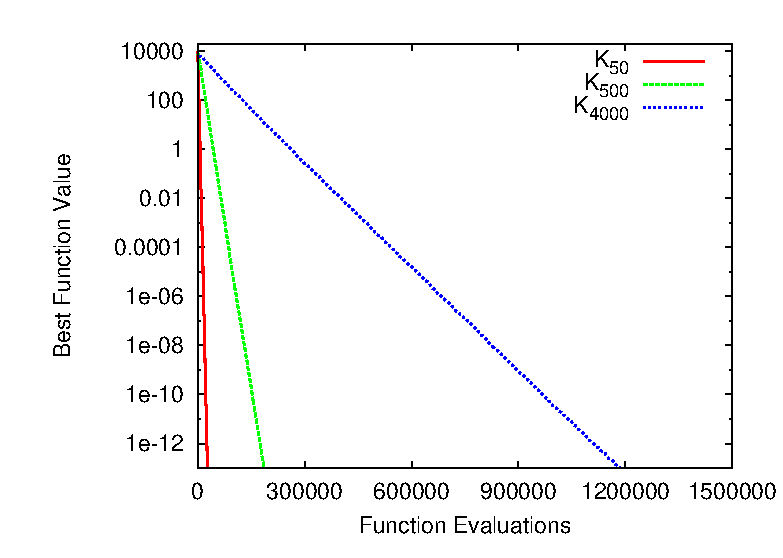
\includegraphics[width=.45\columnwidth]{evals_sphere}
  \caption{Function Sphere with various swarm sizes. Error bars show median and
  10th and 90th percentiles.}
  \label{fig:evals-sphere}
\end{figure}

In this paper we consider PSO parallelization strategies for clusters of
hundreds of processors and functions for which a single evaluation will take
at least seconds, but probably minutes.  Our purpose
is to explore the question of what to do with a hundred processors when 50 or
100 particles is the recommended swarm size, and simply increasing the swarm
size encounters diminishing returns.

To solve this problem, we propose a method for performing two iterations of PSO
at the same time in parallel that we call speculative evaluation.  The name
comes from an analogy to speculative execution (also known as branch
prediction) a technique commonly used in processors.  Modern processors, when
faced with a branch on which they must wait (e.g. a memory cache miss), guess
which way the branch will go and start executing, ensuring that any changes
can be undone.  If the processor guesses right, execution is
much farther ahead than if it had idly waited on the memory reference.  If
it guesses wrong, execution restarts where it would have been anyway.  

In this paper we show that the results of standard PSO can be reproduced
\emph{exactly}, two iterations at a time, using a speculative approach adapted
from speculative execution. We prove that the standard PSO equation can be
factored such that a set of speculative positions can be found which will
\emph{always} include the position computed in the next iteration.  By
computing the value of the objective function for each of the speculative
positions at the same time the algorithm evaluates the objective function for
the current position, it is possible to know the objective function values for
both the current and the next iteration at the same time.  We demonstrate this
principle by implementation and show that it produces exactly the same results
as standard PSO, but two iterations at a time.  The resulting implementation
runs efficiently on large clusters where the number of processors is much
larger than a typical or reasonable number of particles, producing better
results in less ``wall-clock'' time.

The balance of this paper is organized as follows. \sec{pso} describes the
particle swarm optimization algorithm.  \sec{sepso} describes how speculative
evaluation can be done in parallel PSO to perform two iterations at once, then
presents a comparison of the speculative algorithm with the original PSO.  In
\sec{conclusion} we conclude.

\section{Particle Swarm Optimization}
\label{sec:pso}

Particle swarm optimization was proposed in 1995 by James Kennedy and Russell
Eberhart~\cite{kennedy-1995-particle-swarm-optimization}.  The algorithm is
used to intelligently search a multi-dimensional space by mimicking the
swarming and flocking behavior of birds and other animals. It is a social
algorithm that depends on interaction between particles to quickly and
consistently approximate the optimal solution to a given objective function.

The motion of particles through the search space has three components: an
inertial component that gives particles momentum as they move, a cognitive
component where particles remember the best solution they have found and are
attracted back to that place, and a social component by which particles are
attracted to the best solution that any of their neighbors have found.

At each iteration of the algorithm, the position $\ppos_t$ and velocity
$\pvel_t$ of each particle are updated as follows:
\begin{align}
\label{eq:velupdate}
	\pvel_{t+1} &=
		\constriction \bigl[ \pvel_t
			+ \pcoeff\pURand_{t}\otimes(\pbest_{t} - \ppos_{t})
			+ \ncoeff\nURand_{t}\otimes(\nbest_{t} - \ppos_{t})
		\bigr] \\
\label{eq:posupdate}
	\ppos_{t+1} &= \ppos_{t} + \pvel_{t+1}
\end{align}
where \( \pURand_{t} \) and \( \nURand_{t} \) are vectors of independent random
numbers drawn from a standard uniform distribution, the \( \otimes \) operator
is an element-wise vector multiplication, $\pbest$ (called personal best) is
the best position the current particle has seen, and $\nbest$ (called
neighborhood best) is the best position the neighbors of the current particle
have seen~\cite{bratton-2007-defining-a-standard-for-pso}.  The parameters \(
\ncoeff \), \( \pcoeff \), and \( \constriction \) are given prescribed values
required to ensure convergence (2.05, 2.05, and .73,
respectively)~\cite{clerc-2002-constricted-pso}. 

Changing the way neighbors are defined (often called the ``topology'' in the
literature) has a significant effect on the performance of the algorithm.  In
the Ring topology, each particle has one neighbor to either side of it; in the
Complete topology, every particle is a neighbor to every other
particle~\cite{bratton-2007-defining-a-standard-for-pso}.  In all topologies a
particle is also a neighbor to itself in that its own position and value are
considered when updating the particle's neighborhood best, $\nbest$.  Thus with
$p$ particles, using the Ring topology each particle with index $i$ has three
neighbors: $i-1$, $i$ (itself), and $i+1$.  With the Complete topology, each
particle has $p$ neighbors.

In this paper we use these topologies as well as a parallel adaptation of the
Complete topology, called Random, that has been shown to approximate the
behavior of Complete with far less
communication~\cite{mcnabb-2009-large-particle-swarms}.  In the Random
topology, each particle randomly picks two other particles to share information
with at each iteration, along with itself.  Thus in both the Ring and the
Random topologies, all particles have three neighbors.

\section{Speculative Evaluation in PSO}
\label{sec:sepso}

The PSO algorithm can be trivially parallelized by distributing the processing
needed for each particle on across processors.  But as we have seen in
\fig{evals-sphere}, for some functions, and for large numbers of
processors, just adding particles reaches a point of diminishing returns.
That is, adding processors does not help us reach any given level of fitness
appreciably faster.  Instead of adding particles we employ a speculative
evaluation approach that allows us to perform iterations two at a time.

To do so we must first refactor PSO such that the determination of the value
of the objective function is separate from the rest of the computation.  For
simplicity, this discussion will describe the case where PSO is performing
function minimization using the Ring topology.  In this example, each particle
has two neighbors, the ``right neighbor'' and ``left neighbor,'' whose
positions are represented as $\rightn$ and $\leftn$ respectively.  Though we
will only describe the case of the Ring topology, this method can easily be
extended to arbitrary topologies.

The refactoring hinges on the idea that once the random coefficients $\pURand_{t}$ and $\pURand_{t}$ are
determined, there are only a few possible updates to $\nbest$ and $\pbest$.
For the Ring topology there are 7 possible update cases, identified in
Table~\ref{tab:evals}.  We label each case with an identifier referring to the
source of the update: a minus sign ($-$) represents no update, $L$ represents
an update to $\nbest$ coming from the left neighbor, $R$ represents an update
to $\nbest$ coming from the right neighbor, and $S$ represents an update to
either $\pbest$ or $\nbest$ coming from the particle itself.  As an example,
$\casexn$ refers to the case that the particle finds a new personal best, but
neither it nor its neighbors found a position that updated its neighborhood
best.  In the equations that follow, we refer to an unspecified update case as
$\casegen$, and to the set of cases collectively as $\caseset$.

\begin{table}
  \caption{All possible updates for a particle with two neighbors}
  \label{tab:evals}
  \centering
  \begin{tabular}{lcc}
	Identifier&Source of $\pbest$ update&Source of $\nbest$ update\\
	\hline
	\hline
	$\casepn$&No update&No update\\
	\hline
	$\casepl$&No update&Left Neighbor\\
	\hline
	$\casepr$&No update&Right Neighbor\\
	\hline
	$\casexn$&Self&No update\\
	\hline
	$\casexl$&Self&Left Neighbor\\
	\hline
	$\casexr$&Self&Right Neighbor\\
	\hline
	$\casexx$&Self&Self\\
	\hline
  \end{tabular}
\end{table}

In order to incorporate the determination of which case occurs into the
position and velocity update equations, we introduce an indicator function
$\indic_{t+1}^{\casegen}$ for each case $\casegen \in \caseset$.  When
$\casegen$ corresponds to the case taken by PSO,
$\indic_{t+1}^{\casegen}$ evaluates to 1; otherwise it evaluates to 0.  We can
then sum over all of the cases, and the indicator function will make all of the
terms drop to zero except for the case that actually occurs.  For example, the
indicator function for the specific case $\casexn$ can be written as follows:
\begin{align}
  \nonumber
	&\indic_{t+1}^{\casexn}\parens{
	  \ofunc\parens{\ppos_{t}},
	  \ofunc\parens{\leftn_{t}},
	  \ofunc\parens{\rightn_{t}},
	  \ofunc\parens{\pbest_{t-1}},
	  \ofunc\parens{\nbest_{t-1}}
	  } \\
  &\hspace{15pt}= \label{eq:deficasexn}
	\begin{cases}
	  1 & \text{if}~
		\ofunc\parens{\ppos_{t}} < \ofunc\parens{\pbest_{t-1}}
	    \,\text{and}\,
		\ofunc\parens{\nbest_{t-1}} < \min\parens{
		  \ofunc\parens{\ppos_{t}},
		  \ofunc\parens{\leftn_{t}},
		  \ofunc\parens{\rightn_{t}}
		} \\
	   0 & \text{otherwise}
	\end{cases}
\end{align}

For each case $\casegen \in \caseset$, there is also a corresponding
velocity update function $\specvel_{t+1}^{\casegen}$.  When the case is
known, the specific values of $\pbest_t$ and $\nbest_t$ may be substituted
directly into~\eqref{eq:velupdate}.  For example, in case $\casexn$,
$\pbest_{t}=\ppos_{t}$, as \pbest was updated by the particle's current
position, and $\nbest_{t}=\nbest_{t-1}$, as $\nbest$ was not updated at
iteration $t$:
\begin{align}
\nonumber
	\specvel_{t+1}^{\casexn} & \parens{\pvel_t, \ppos_{t}, \leftn_{t}, \rightn_{t},
	\pbest_{t-1}, \nbest_{t-1}, \pURand_{t}, \nURand_{t}} \\
\label{eq:defvcasexn}
		&= \constriction \left[ \pvel_{t} +
			\pcoeff\pURand_{t}\otimes\parens{\ppos_{t} - \ppos_{t}}
			+ \ncoeff\nURand_{t}\otimes\parens{\nbest_{t-1} -
			\ppos_{t}} \right]
\end{align}

In the same way we can create notation for the position update function by
substituting into~\eqref{eq:posupdate}:
\begin{align}
    \nonumber
	\specpos_{t+1}^{\casegen} & \parens{\ppos_{t}, \pvel_{t}, \leftn_{t},
	\rightn_{t} ,\pbest_{t-1} ,\nbest_{t-1}, \pURand_{t}, \nURand_{t}}
        \\
    \label{eq:defpcasegen}
        &=
	\ppos_{t} + \specvel_{t+1}^{\casegen}
	\parens{\pvel_t, \ppos_{t}, \leftn_{t}, \rightn_{t},
	\pbest_{t-1}, \nbest_{t-1}, \pURand_{t}, \nURand_{t}}
\end{align}

With this notation we can re-write the original PSO velocity
equation~\eqref{eq:velupdate}, introducing our sum over cases with the
indicator functions.
The velocity~\eqref{eq:velupdate} and position~\eqref{eq:posupdate} equations become:
\begin{align}
\nonumber
  \pvel_{t+1} &= \sum_{c \in \caseset} \bigl[
	\indic_{t+1}^{c}\parens{
	  \ofunc\parens{\ppos_{t}},
	  \ofunc\parens{\leftn_{t}},
	  \ofunc\parens{\rightn_{t}},
	  \ofunc\parens{\pbest_{t-1}},
	  \ofunc\parens{\nbest_{t-1}}
	  } \\
\label{eq:specvelupdate}
	& \quad \quad \quad \specvel_{t+1}^{c}\parens{
	  \ppos_{t},
	  \pvel_{t},
	  \leftn_{t},
	  \rightn_{t},
	  \pbest_{t-1},
	  \nbest_{t-1},
	  \pURand_{t},
	  \nURand_{t}
	  }\bigr]
\\
\nonumber
  \ppos_{t+1} &= \sum_{c \in \caseset} \bigl[
	\indic_{t+1}^{c}\parens{
	  \ofunc\parens{\ppos_{t}},
	  \ofunc\parens{\leftn_{t}},
	  \ofunc\parens{\rightn_{t}},
	  \ofunc\parens{\pbest_{t-1}},
	  \ofunc\parens{\nbest_{t-1}}
	  } \\
\label{eq:specposupdate}
	& \quad \quad \quad \specpos_{t+1}^{c}\parens{
	  \ppos_{t},
	  \pvel_{t},
	  \leftn_{t},
	  \rightn_{t},
	  \pbest_{t-1},
	  \nbest_{t-1},
	  \pURand_{t},
	  \nURand_{t}
	  }\bigr]
\end{align}

In this form the important point to notice is that there are only $7$ values
(for this Ring topology) in the set $\{\specpos_{t+1}^{\casegen}: \casegen \in
\caseset\}$ and that none of them depend upon $f(\ppos_t)$ or any other
objective function evaluation at iteration $t$. Note also that while there are
random numbers in the equation, they are assumed fixed once drawn for any
particular particle at a specific iteration.  Thus PSO has been refactored such
that the algorithm can begin computing all $7$ of the objective function
evaluations potentially needed in iteration $t+1$ \emph{before} $f(\ppos_t)$ is
computed.  Once the evaluation of $f(\ppos_{t})$ is completed for all particles
only one of the indicator functions $\indic_{t+1}^{\casegen}$ will be set to 1;
hence only one of the positions $\specpos_{t+1}^\casegen$ will be kept.

Although this speculative approach computes
$\ofunc(\specpos_{t+1}^{\casegen})$ for all $\casegen \in \caseset$, even those
for which $\indic_{t+1}^{\casegen} = 0$, these extra computations will be
ignored, and might just as well never have been computed.  We call the set of
computations $\{\ofunc(\specpos_{t+1}^{c}) : \casegen \in \caseset\}$
``speculative children'' because only one of them will be needed.

To see the value of this refactoring, suppose that $800$ processors are
available, and that the evaluation of the function to be optimized takes one
hour.  If we only want a swarm of $100$ particles, $700$ of the processors
would be sitting idle for an hour at every iteration, and it would take two
hours to run two iterations.  If instead we perform speculative evaluation,
sending each of the $\ofunc(\specpos_{t+1}^{c})$ to be computed at the same
time as $\ofunc(\ppos_{t})$, we could create a swarm of size 100, each particle
with $7$ speculative evaluations ($700$ processors dedicated to speculative
evaluation), thus using all $800$ processors and performing two iterations in
one hour.

In order to do two iterations at once, we use 8 times as many processors as
there are particles in the swarm.  If these processors were not performing
speculative evaluation, they might instead be used for function evaluation
needed to support a large swarm.  This raises the question of whether a swarm
of 100 particles doing twice as many iterations outperforms a swarm of 800
particles.  We show in the rest of this paper that in many, instances, a
smaller swarm performing more iterations does in fact outperform a larger
swarm.  We acknowledge that both intuition and prior
research~\cite{mcnabb-2009-large-particle-swarms} indicate that the
optimization of deceptive functions benefits greatly from large and even very
large swarm sizes. Thus this work will focus on less deceptive functions.

\subsection{Implementation}
\label{sec:implementation}

The number of speculative evaluations needed per particle depends on the number
of neighbors each particle has.  In a swarm with $p$ particles and $n$
neighbors per particle, $(2n+1)p$ speculative evaluations are necessary (each
additional neighbor adds two rows to Table~\ref{tab:evals}).  This dependence
on the number of neighbors necessitates a wise choice of topology.  The use of
the Complete topology, where every particle is a neighbor to every other
particle, would require $O(p^2)$ speculative evaluations per iteration.  It is
much more desirable to have a sparse topology, where $O(np)$ is much smaller
than $O(p^2)$.  However, some functions are better optimized with the Complete
topology and the quick spread of information it entails than with sparse
topologies.  In such cases, we use the Random topology described in \sec{pso}.

To aid in describing our implementation, we introduce a few terms. We use
$\p_t$ to denote a particle at iteration $t$ and $\s_{t+1}$ to denote one of
$\p_t$'s speculative children, corresponding to one of the rows in
Table~\ref{tab:evals}.  $\n_t$ is a neighbor of particle $\p_t$.  Sets of
particles are given by $\pset$, $\sset$, or $\nset$, whereas single particles
are simply $\p$, $\s$, or $\n$.

A particle at iteration $t-1$ that has been moved to iteration $t$ using
\eqref{eq:velupdate}~and~\eqref{eq:posupdate}, but whose position has not yet
been evaluated, is denoted as $\noeval{\p}_t$.  Once its position has been
evaluated, but it has still not yet received information from its neighbors, it
is denoted as $\nonbest{\p}_t$.  Only when the particle has updated its
neighborhood best is it a complete particle at iteration $t$.  It is then
simply denoted as $\p_t$.

The outline of the speculative evaluation in PSO (SEPSO) algorithm is given in
\alg{centralized}.

\begin{algorithm}
  \caption{Speculative Evaluation PSO (SEPSO)}
  \label{alg:centralized}
  \begin{algorithmic}[1]
	\STATE Move all $\p_{t-1}$ to $\noeval{\p}_t$ using
	  \eqref{eq:velupdate}~and~\eqref{eq:posupdate}
	\STATE For each $\noeval{\p}_t$, get its neighbors $\noeval{\nset}_t$ and
	  generate $\noeval{\sset}_{t+1}$ according to
	  \eqref{eq:defpcasegen}.
	\STATE Evaluate all $\noeval{\p}_t$ and $\noeval{\sset}_{t+1}$ in parallel
	\STATE Update personal best for each $\noeval{\p}_t$ and
	  $\noeval{\s}_{t+1}$, creating $\nonbest{\p}_t$ and $\nonbest{\s}_{t+1}$
	\STATE Update neighborhood best for each $\nonbest{\p}_t$, creating
	  $\pset_t$
	\FORALL{$\p_t$}
	\STATE Pick $\nonbest{\s}_{t+1}$ from $\nonbest{\sset}_{t+1}$ that matches
	  the branch taken by $\p_t$ according to
	  \eqref{eq:specposupdate}.
	\STATE Pass along personal and neighborhood best values obtained by $\p_t$,
	  making $\nonbest{\p}_{t+1}$
	\ENDFOR
	\STATE Update neighborhood best for each $\nonbest{\p}_{t+1}$, creating
	  $\pset_{t+1}$
	\STATE Repeat from Step 1 until finished
  \end{algorithmic}
\end{algorithm}

\section{Using All Speculative Evaluations}
\label{sec:extra}

In performing speculative evaluation as we have described it, $2n+1$
speculative evaluations are done per particle, while all but one of them are
completely ignored.  It seems reasonable to try to make use of the
information obtained through those evaluations instead of ignoring it
Making use of this information changes the
behavior of PSO, instead of reproducing it exactly as the above method
explains, but the change turns out to be an improvement in our context.

To make better use of the speculative evaluations, instead of choosing the speculative
child that matches that branch that the original PSO would have taken, we take
the child that has the best value.  The methodology is exactly the same as
above except for the process of choosing which speculative child to accept.
The branch that PSO would have taken is ignored, but $\p_t$ must still be
created so it can give the right personal best and neighborhood best values and
positions to $\p_{t+1}$.  The only change needed in \alg{centralized} is in
step 7, where the $\noeval{\s}_{t+1}$ with the best value is chosen from
$\noeval{\sset}_{t+1}$ instead of with the matching branch. We call this
varient ``Pick Best''.

This can be thought of as drawing a number of samples from the next iteration
and accepting the best one.  Speculative particles that move in good directions
are kept.  It seems this modification to PSO would contribute local exploration,
having knowledge of all of the speculative children, but more global exploitation,
since Pick Best only considers the best of these alternatives.
With functions that are less deceptive, or only locally deceptive,
Pick Best works well, while performance on more deceptive
functions would probably be hurt.

\section{Results}
\label{sec:results}

In our experiments we compared our speculative PSO algorithm to the standard
PSO algorithm.  At each iteration of the algorithms, we use one processor to
perform one function evaluation for one particle, be it speculative or
non-speculative.  The speculative algorithm actually performs two iterations of
PSO at each ``iteration,'' so we instead call each ``iteration'' a round of
evaluations.  For benchmark functions with very fast evaluations this may not
be the best use of parallelism in PSO.  But for many real-world applications,
the objective function takes on the order of at least seconds (or more) to evaluate; in
such cases our assumption is perfectly reasonable.

In each set of experiments we keep the number of processors for each algorithm constant.
In all of our SEPSO experiments each particle has
two neighbors in addition to itself.
As shown in
Table~\ref{tab:evals}, this results in $7$ speculative evaluations per
particle.  With one evaluation needed for the original, non-speculative
particle, we have a total of $8p_s$ evaluations for every two iterations, where $p_s$ is
the number of particles in the speculative swarm.
We run these experiments on $8p_s$ processors.
In the base-line experiments, standard pso the same number of processors and thus enjoys the
benefit of $8p_s$ particles running on 
$8p_s$ processors.
At least in benchmark functions, extra particles only accelerate
the performance of PSO~\cite{mcnabb-2009-large-particle-swarms}. They generally have diminishing value, as
seen earlier in \fig{evals-sphere}, but these extra particles give standard PSO the best possible
context and full access to the same resources as SEPSO.

As discussed in \sec{implementation},
where the Complete topology would normally be used, we use a Random topology in
our speculative algorithm, as Complete leads to an explosion of speculative
evaluations.
For the standard PSO baseline we have included experiments with the
ring and the random topologies, both with two neighbors, as well as for the complete topology.
It is important to note however, that in many cases the complete topology is not a
practical alternative in the context of large
swarms on large cluster where where the messaging complexity is $O(n^2)$ and can
overwhelm the system.

We follow the experimental set up proposed by Bratton, et.al.~\cite{bratton-2007-defining-a-standard-for-pso}. 
All functions have 20 dimensions, and all results shown
are averages over 20 runs.  We use 240 processors in our experiments, so
speculative algorithms use 30 particles and standard PSO uses 240 particles.
For ease of labeling, we call our speculative algorithm SEPSO, the variant
SEPSO Pick Best, and standard PSO just PSO and identify the topology in a suffix,
``PSO Ring'' for example.

The benchmark function Sphere ($f(\Vec{x}) = \sum_{i=1}^D x_i^2$)
has no local optima and is most efficiently optimized using
a small swarm but many iterations.
In \fig{sphere1}, we can see
that SEPSO clearly beats PSO with a Random topology or a ring topology.

SEPSO approaches the performance of PSO with the complete topology, even though
PSO with the complete topology requires $O(n^2)$ communication.
SEPSO Pick Best handily outperforms all other algorithms
in this problem.

\begin{figure}
  \centering
  \includegraphics[width=.45\columnwidth]{sphere1}
  \caption{Function Sphere with a swarm that uses 240 processors per round of
  evaluations.  Speculative algorithms have a swarm of 30 particles and do two
  iterations per round, while standard PSO algorithms use 240 processors and do
  one iteration per round. Note that PSO Complete requires $O(n^2)$ messaging
  and may not be practical in many cases.}
  \label{fig:sphere1}
\end{figure}

The benchmark function Griewank, defined by the equation $f(\Vec{x}) =
\frac{1}{4000} \sum_{i=1}^D x_i^2 - \Pi_{i=1}^D \cos\left(\frac{x_i}{\sqrt{i}}
\right) + 1$.  It is generally best solved in pso using the Ring topology,
as Complete is prone to premature convergence
on a local optimum.  Griewank has a global optimum with a value of 0, and
sometimes the swarm finds the optimum and sometimes it does not.  Instead of
showing average function value at each iteration, a more enlightening plot for
Griewank shows the percent of runs that have found the global optimum by each
iteration~\cite{bratton-2007-defining-a-standard-for-pso}. 

PSO and SEPSO get caught in local minima with small swarm sizes so
we show results in \fig{griewank1} for swarms of size 100 (SEPSO) and 800 (standard)
using the Ring topology 
\fig{griewank2} shows that SEPSO quickly finds
the global optimum essentially 100\% of the time.

\begin{figure}
  \centering
  \includegraphics[width=.45\columnwidth]{griewank2}
  \caption{Function Griewank with a swarm that uses 800 processors per round of
  evaluations.}
  \label{fig:griewank2}
\end{figure}

As noted in the introduction previous work has shown that the optimization of highly
deceptive functions like Rastrigin
($f(\Vec{x}) = \sum_{i=1}^D \left(x_i^2 - 10\cos\left(2\pi x_i\right) + 10\right)$)
benefit greatly from the addition of particles. 
Smaller swarms get caught
in local optima.  Because our speculative algorithms have a significantly
smaller swarm size, they get stuck at higher values while the larger swarms
performing regular PSO continue to improve the best value found.
Our experiments with SEPSO on Rastrigin were predicable lack luster,
yielding a vaerage value of xxx after x evaluations, as compared to y for 
standard PSO.

\section{Conclusions}
\label{sec:conclusion}

We have described how parallel implementations of particle swarm optimization
can be modified to allow additional processors to increase the number of
iterations of the algorithm performed, instead of merely adding more particles
to the swarm.  We have detailed several different implementations of the
algorithm, depending on the parallel PSO framework being used.  Using our
modifications, the original PSO algorithm is exactly reproduced two iterations
at a time.  This technique requires more function evaluations per iteration
than regular PSO, but for some functions still performs better when run in a
parallel environment.

We have also described a method for making use of extra speculative evaluations
that performs incredibly well on some functions.

Though space has limited our presentation of results to a very small sample of
the interesting and relevant applications of our technique, we believe the
results shown are sufficient motivation for the further exploration of
speculative evaluation in PSO.

Our results show that performing speculative evaluation instead of increasing
swarm size is only beneficial for some functions at the swarm sizes we used.
However, we would venture that for all functions there is some point at which
increasing the swarm size provides relatively little benefit.  At that point,
additional processors should be used to speed up the algorithm instead of add
additional particles.

There are some functions for which very little exploration needs to be done;
Sphere is an example of such a function.  For such functions the best use of
processors is to have a small swarm performing speculative evaluation with our
second method, where all speculative evaluations are used.

There are other functions for which there is a point where the algorithm has
done ``enough'' exploration and consistently finds the global optimum.  Adding
additional particles to the swarm is akin to increasing its capacity for
exploration.  We have seen that for a 20-dimensional Griewank function, 30
particles is not ``enough'' exploration, but 100 is.  For these functions, one
should use processors to increase the swarm size until enough exploration has
been reached, then use additional processors to increase the number of
iterations performed.

There are still other functions for which it seems there is never enough
exploration, such as the Rastrigin function.  It has been shown that up to 4000
particles there is no point at which ``enough'' exploration has been
done~\cite{mcnabb-2009-large-particle-swarms}.  For those functions the correct
use of processors cannot be easily prescribed and depends largely on the
desired outcome and how many processors are available.  It is likely that the
best thing to do with those functions is to use all processors to add particles
to the swarm and do no speculative evaluation.

\bibliographystyle{unsrt}
\bibliography{%
../../../bib/aml/bib,%
../../../bib/pso/general/bib,%
../../../bib/pso/parallel/bib,%
../../../bib/pso/topology/bib,%
../../../bib/sim-anneal/parallel/bib,%
../../../bib/ga/bib}
\end{document}
